\documentclass[../main.tex]{subfiles}
\begin{document}
\chapter{The Double-$\tau_h$ + jet trigger}

In view of Run 3, a lot of effort has been dedicated in order to maximize the collection efficiency from physics processes with much smaller cross sections than the backgrounds, as is the case for both H~$\to\tau\tau$ and HH~$\to$~bb$\tau\tau$ processes. In these two cases, in most events the produced $\tau\tau$ pair is accompanied by one or more jets coming from the hard-scattering processes or from QCD radiation (in addition to the 2 $b$-jets coming from the other H in the HH~$\to$~bb$\tau\tau$ process), as seen in Fig.~\ref{hh:fig:trig_ngenjets}.

Therefore, by including in the menu a new trigger that requires two $\tau_h$ and an additional jet (whose $p_t$ spectre is shown in Fig.~\ref{hh:fig:trig_l1jet_pt}), the $p_t$ threshold on the $\tau_h$ could be lowered. By doing so, as more $\tau_h$ will be available for triggering (see Fig.~\ref{hh:fig:trig_l1tau_pt}), the acceptance of both analyses could be enlarged.


\begin{figure}[h!]
\begin{center}
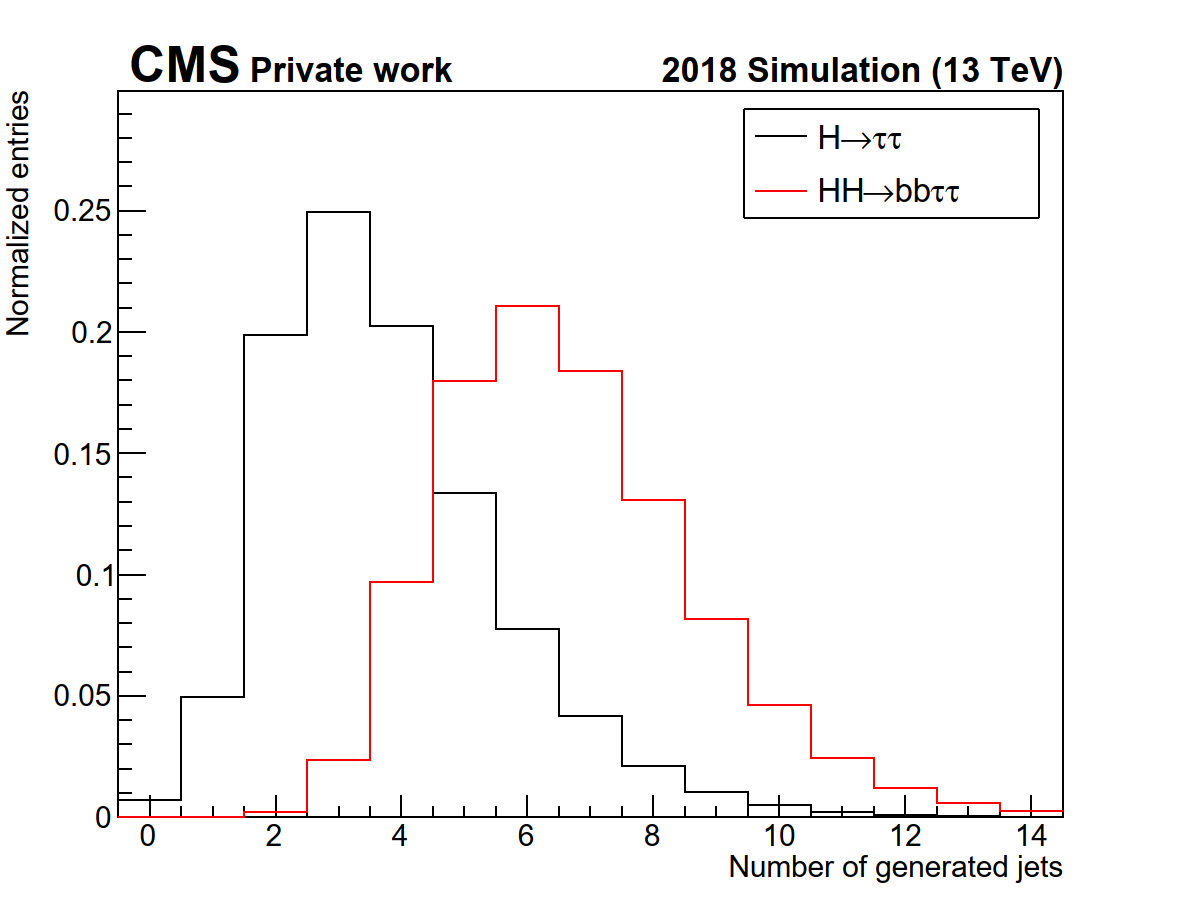
\includegraphics[width=0.6\textwidth]{Images/ngenjets}
\end{center}
\caption{Number of jets  per event at generator level for H~$\to\tau\tau$ (black) and HH~$\to$~bb$\tau\tau$ ggHH (red) processes, both produced via ggF.}
\label{hh:fig:trig_ngenjets}
\end{figure}

\begin{figure}[h!]
\begin{center}
\includegraphics[width=0.5\textwidth]{Images/leading_jet_pt}
\end{center}
\caption{L1 leading jet $p_t$ for the H~$\to\tau\tau$ (black) and HH~$\to$~bb$\tau\tau$ (red) processes, both produced via ggF.}
\label{hh:fig:trig_l1jet_pt}
\end{figure}

\begin{figure}[h!]
\begin{center}
\subfloat{\includegraphics[width=0.5\textwidth]{Images/l1tau_pt_htt_ggf_new}}
\subfloat{\includegraphics[width=0.5\textwidth]{Images/l1tau_pt_hhbbtt_ggf_new}}
\end{center}
\caption{L1 leading and subleading $\tau_h$ $p_t$ for the H~$\to\tau\tau$ (left) and HH~$\to$~bb$\tau\tau$ (right) processes, both produced via ggF.}
\label{hh:fig:trig_l1tau_pt}
\end{figure}

In the following sections we will discuss the design and performance of a new L1 seed with two $\tau_h$ and one jet to be included in the L1 Menu and a new HLT path seeded by this new L1 seed. The goal is that the newly defined L1 seed and HLT path add as little rate as possible but increasing the final acceptance on the H~$\to\tau\tau$ and HH~$\to bb\tau\tau$ analysis. This acceptance will come not only from the new trigger, but also from the corresponding changes on the offline selections. In the $H\to\tau\tau$ analysis \cite{hh:htt_run2}, the two $\tau_h$ are selected if their $p_T > 40$~GeV, while the selection on the jets varies depending on the category considered among four different categories. In the following study we will consider two categories, obtained as a simplification of the original analysis categories: the 1-jet, high $p_t$ category, where we consider events with one jet with $p_T > 70$~GeV; and the 2-jet category, where we select events with two jets with $p_T > 30$~GeV. In the HH~$\to$~bb$\tau\tau$ category, as was described in Chapter~\ref{hh:chapter:analysis}, events with two $\tau_h$ with $p_t>40$~GeV and two jet candidates with $p_t>20$~GeV are selected.



\section{The L1 Double-$\tau_h$ + jet trigger}
\label{hh:sec:l1seeds}

In the L1 menu used during the Run-2 data taking, the only seeds that consider hadronic $\tau$ decays were the \texttt{L1\_DoubleIsoTauXer2p1} seeds, where two isolated $\tau_h$ with $p_t\geq X$~GeV and $|\eta|<2.1$ are selected. The threshold $X$ varied during the data-taking, with a value of $X=32~$GeV during 2018. The strategy we will follow in this study is to include a new seed in the L1 Menu with two isolated $\tau_h$ objects and one jet object identified by the $\mu$GT. This way, it could complement the already present double-$\tau_h$ seed with the same 32~GeV threshold (or with a larger $p_t$ threshold in order to keep the rate as low as possible). However, a particular treatment has to be given to seeds involving $\tau_h$ and jet objects simultaneously, as both, $\tau_h$ and jets, are reconstructed as purely calorimetric objects. Then, all $\tau_h$ objects will enter the L1 jet collection, while some of the L1 jets will also appear in the L1 $\tau_h$ collection. This issue can be perfectly seen in Fig.~\ref{hh:fig:l1_tau_jet_dR}. To reduce this effect, a feature called overlap removal \cite{intro:l1_13tev} is used, so only L1 jets that are separated more than $\Delta R>0.5$ with the selected $\tau_h$ are considered. This feature was present in the $\mu$GT before the inclusion of the seeds, although none of the already present seeds were using it and, in fact, it had to be tuned and validated before attempting the inclusion of the new seeds.

\begin{figure}[h!]
\begin{center}
\includegraphics[width=0.5\textwidth]{Images/l1_tau_jet_dR}
\end{center}
\caption{Minimal $\Delta R$ between all L1 $\tau_h$'s and jets per event in a $H\to\tau\tau$ ggH simulated sample. The peak appearing at small $\Delta R$ values is due to the overlap between the L1 $\tau_h$ and jet collections.}
\label{hh:fig:l1_tau_jet_dR}
\end{figure}

As previously stated, this new double-$\tau_h$+jet seed (encoded as \texttt{L1\_Double\-IsoTauY\-er2p1\-\_JetZ\_RmOvlp\_dR0p5}, where $Y$ and $Z$ are the $p_T$ thresholds for the $\tau_h$ and jet, respectively) does not aim to replace the present \texttt{L1\_Double\-Iso\-Tau32er2p1} seed, but to complement it. However, in order to make some rate available for the new seed, increasing the double-$\tau_h$ $p_T$ threshold to a value $X$ could be needed. The rates corresponding to different values of the double-$\tau_h$ threshold are shown in Fig.~\ref{hh:fig:trig_ditau32_rate}. These rates are estimated using a zero bias data sample (where the only requirement is that two bunches have collided) taken during a 2018 run but with Run-3 conditions applied (PU linearly scaled to 53 and 2748 colliding bunches). After the inclusion of the new seed, the aim is to keep the total rate of both seeds as close as possible to the rate coming from the \texttt{L1\_Double\-Iso\-Tau32er2p1} seed, so a target rate of $\sim17$~kHz will be considered.

\begin{figure}[h!]
\begin{center}
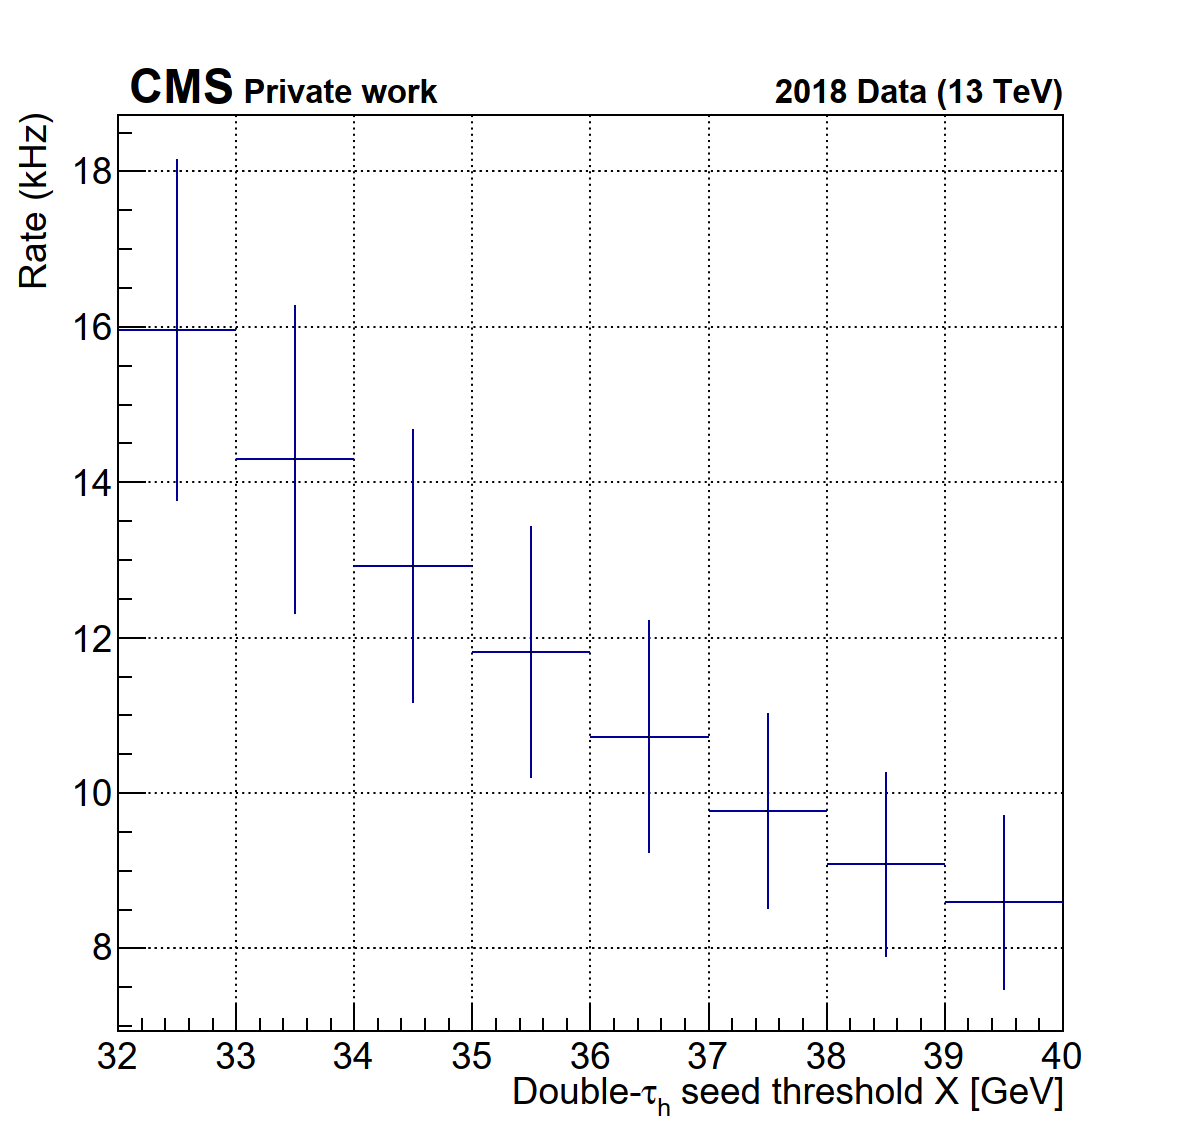
\includegraphics[width=0.5\textwidth]{Images/plot2D_ditau_sym_323755}
\end{center}
\caption{Rate of the \texttt{L1\_DoubleIsoTauXer2p1} trigger seed as a function of the $X$ threshold.}
\label{hh:fig:trig_ditau32_rate}
\end{figure}

As we would like to increase the signal acceptance, we will compute the acceptance gain when considering the two new seeds instead of the reference \texttt{L1\_Double\-IsoTau32\-er2p1} seed. In this case we will consider four signal samples, two ggF and VBF H~$\to\tau\tau$ and two ggF and VBF HH~$\to$~bb$\tau\tau$. These acceptance gains are computed not only from the L1 objects that pass the required selection cuts (grouped in the booleans \texttt{PassL1DoubleTau32}, \texttt{PassL1DoubleTauX} and \texttt{PassL1DoubleTauYJetZ}), but also applying selections to the objects obtained by the offline reconstruction system that evolve accordingly to the L1 thresholds considered. In general, this evolution means that, for a given L1 $p_t$ threshold $T$, the offline threshold is obtained as $T$ + $\Delta T$. As in both target analysis the offline threshold is set to 40~GeV when using a L1 threshold of 32~GeV, we will consider $\Delta T=8$~GeV for the $\tau_h$. For the jets we will consider $\Delta T=10$~GeV. All $p_t$ selections are summarised in Table~\ref{hh:tab:trig_offpt}, where one boolean associated to each seed has been defined to group the needed selections. On top of these $p_t$ cuts, all offline jets must be within $|\eta|<4.7$ and pass tight jet ID and loose PU jet ID and an overlap removal criteria with the offline $\tau_h$.

\begin{table}
	\begin{center}
	\begin{tabular}{c || c | c | c }
		                           & \multicolumn{3}{c}{Offline $p_t$ selections} \\
		Boolean                    & 1-jet, high $p_t$ & 2-jet & bb$\tau\tau$ \\\hline\hline
		\texttt{PassOfflDoubleTau32} & 
			$\begin{matrix}
				p_t^{\tau_1}>40\\
				p_t^{\tau_2}>40\\
				p_t^{j_1}>70
			\end{matrix}$ &
			$\begin{matrix}
				p_t^{\tau_1}>40\\
				p_t^{\tau_2}>40\\
				p_t^{j_1}>30 \\
				p_t^{j_2}>30
			\end{matrix}$ &
			$\begin{matrix}
				p_t^{\tau_1}>40\\
				p_t^{\tau_2}>40\\
				p_t^{j_1}>20\\
				p_t^{j_2}>20
			\end{matrix}$ \\\hline
		\texttt{PassOfflDoubleTauX} & 
			$\begin{matrix}
				p_t^{\tau_1}>X+8\\
				p_t^{\tau_2}>X+8\\
				p_t^{j_1}>70
			\end{matrix}$ &
			$\begin{matrix}
				p_t^{\tau_1}>X+8\\
				p_t^{\tau_2}>X+8\\
				p_t^{j_1}>30 \\
				p_t^{j_2}>30
			\end{matrix}$ &
			$\begin{matrix}
				p_t^{\tau_1}>X+8\\
				p_t^{\tau_2}>X+8\\
				p_t^{j_1}>20\\
				p_t^{j_2}>20
			\end{matrix}$ \\\hline
		\texttt{PassOfflDoubleTauYJetZ} &
			$\begin{matrix}
				p_t^{\tau_1}>Y+8\\
				p_t^{\tau_2}>Y+8\\
				p_t^{j_1}>Z+10 \\
				p_t^{j_1}>70
			\end{matrix}$ &
			$\begin{matrix}
				p_t^{\tau_1}>Y+8\\
				p_t^{\tau_2}>Y+8\\
				p_t^{j_1}>Z+10 \\
				p_t^{j_1}>30 \\
				p_t^{j_2}>30
			\end{matrix}$ &
			$\begin{matrix}
				p_t^{\tau_1}>Y+8\\
				p_t^{\tau_2}>Y+8\\
				p_t^{j_1}>Z+10 \\
				p_t^{j_1}>20 \\
				p_t^{j_2}>20
			\end{matrix}$
	\end{tabular}
	\end{center}

	\caption{Offline $p_t$ selections associated to the L1 selections of \texttt{L1\_DoubleIsoTau32er2p1}, \texttt{L1\_DoubleIsoTauXer2p1} and \texttt{L1\_DoubleIsoTauYer2p1\_JetZ\_RmOvlp\_dR0p5}, where $\tau_1$ and $\tau_2$ are the leading and subleading $\tau_h$ and $j_1$ and $j_2$ are the leading and subleading jets. All thresholds are expressed in GeV.}
	\label{hh:tab:trig_offpt}
\end{table}


Thus, the acceptance gain when adding a double-$\tau_h$+jet seed and modifying the threshold of the present double-$\tau_h$ seed can be defined as
\begin{equation}
g(X, Y, Z) = \frac{\begin{matrix}N[(\text{\texttt{PassL1DoubleTauX}} \,\,\&\&\,\, \text{\texttt{PassOfflDoubleTauX}}) \,\,||\,\, \\ \qquad\qquad\qquad(\text{\texttt{PassL1DoubleTauYJetZ}} \,\,\&\&\,\, \text{\texttt{PassOfflDoubleTauYJetZ}})] \end{matrix}}{N[\text{\texttt{PassL1DoubleTau32}} \,\,\&\&\,\, \text{\texttt{PassOfflDoubleTau32}}]}
\end{equation}
where $N$ is the number of events that pass the conditions required for given values of the $X$, $Y$ and $Z$ $p_T$ thresholds. The average acceptance gains obtained for different sets of thresholds ($X$, $Y$, $Z$) for the samples and categories considered is shown in Fig.~\ref{hh:fig:l1_trig_mean_acc} (only the 20 sets with the highest acceptance gain in a 15-17 kHz rate range are displayed). Given these results, the decision was to consider thresholds $Y=26$ and $Z=55$ GeV for the double-$\tau_h$+jet seed, i.e. adding the seed encoded as \texttt{L1\_DoubleIsoTau26er2p1\_Jet55\_RmOvlp\_dR0p5}. In addition, another double-$\tau_h$+jet seed with thresholds $Y=26$ GeV and $Z=70$ GeV was added as a backup seed in case the rate coming from the main seed ends up being larger than expected. Rates for these new seeds and their main acceptance gains on top of the \texttt{L1\_DoubleIsoTau32er2p1} seed for the two processes considered are shown in Table~\ref{hh:tab:l1trig:allseeds}.

\begin{figure}
\subfloat{\centering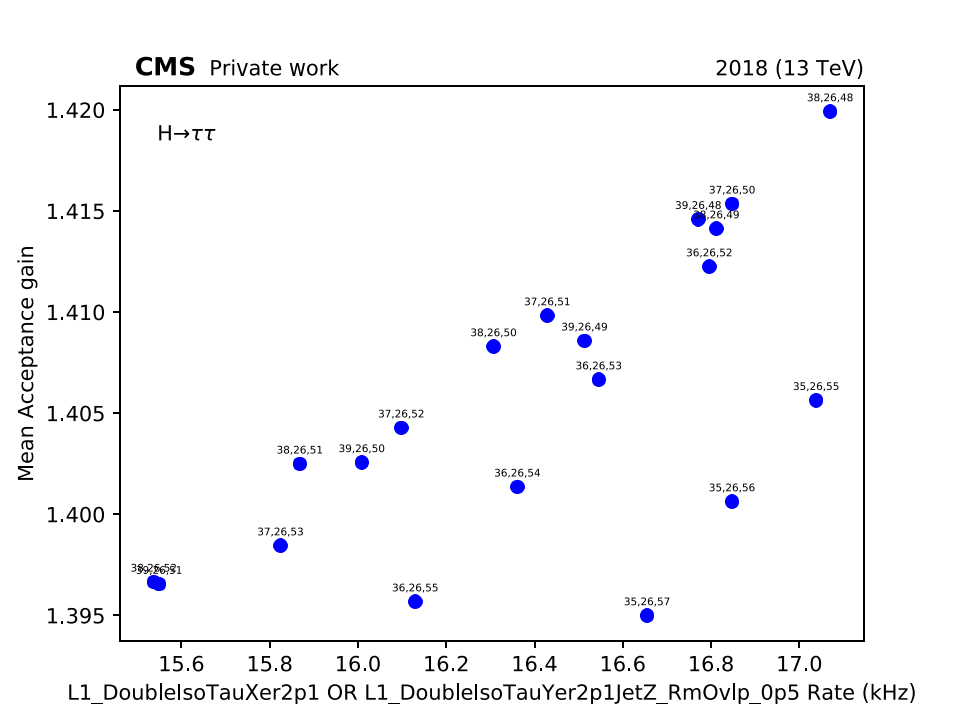
\includegraphics[width=0.49\textwidth]{Images/rate_vs_mean_acceptance__min5.0___max17.1___xx_sym__yy_sym_htt.pdf}}
\subfloat{\centering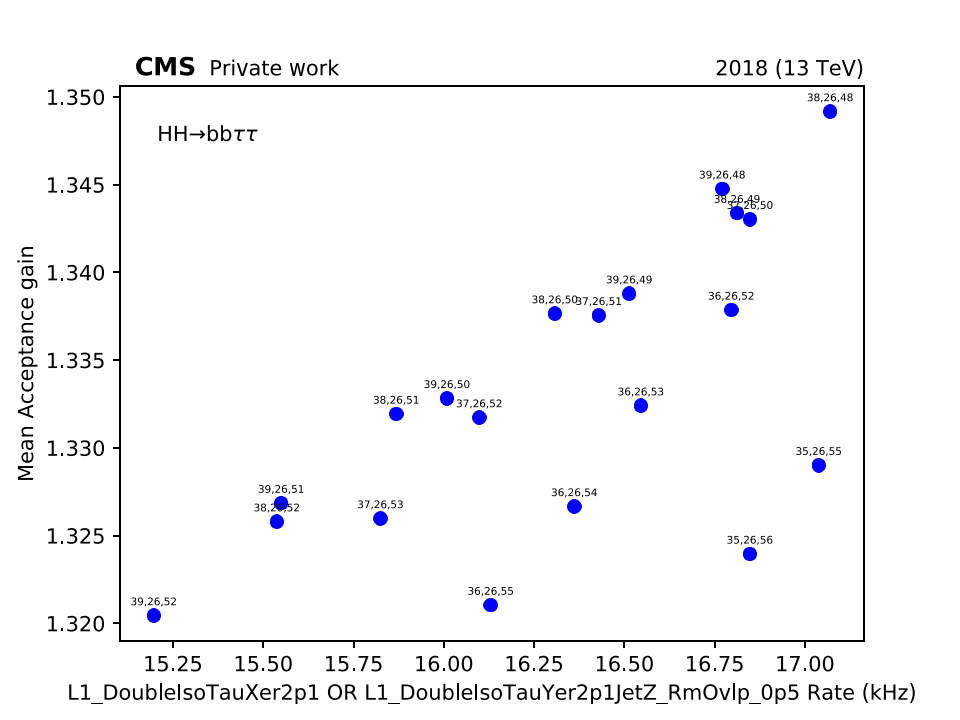
\includegraphics[width=0.49\textwidth]{Images/rate_vs_mean_acceptance__min5.0___max17.1___xx_sym__yy_sym_hhbbtt.pdf}}
\caption{Mean acceptance gain for the H~$\to\tau\tau$ (left) and HH~$\to$~bb$\tau\tau$ (right) processes when considering the new trigger strategy. \textcolor{red}{(probably need to improve plots, e.g. add processes in them)}}
\label{hh:fig:l1_trig_mean_acc}
\end{figure}

\begin{table}[h!]
\begin{small}
\begin{center}
\begin{tabular}{|l|r|r|r|}
\hline
Trigger seed & \multicolumn{2}{c|}{Acceptance gain} &  Rate (kHz) \\
\hline\hline
& H~$\to\tau\tau$ & HH~$\to$~bb$\tau\tau$ &  \\\hline
\texttt{L1\_DoubleIsoTau26er2p1\_Jet55\_RmOvlp\_dR0p5} & 44$\%$ & 36$\%$& $8.3 \pm 2.8$ \\
\texttt{L1\_DoubleIsoTau26er2p1\_Jet70\_RmOvlp\_dR0p5} & 34$\%$ & 29$\%$ & $5.3 \pm 1.8$ \\\hline
\end{tabular}
\end{center}
\end{small}

\caption{Rates and mean acceptance gains for the two new double-$\tau_h$+jet seeds.}
\label{hh:tab:l1trig:allseeds}
\end{table}

%\begin{tabular}{|l|r|rr|rr|rr|r|}
%\hline
%\multicolumn{2}{|r|}{} & \multicolumn{2}{r|}{$H\to\tau\tau$, 1-jet, high $p_t$ cat.} & \multicolumn{2}{r|}{$H\to\tau\tau$, 2-jet cat.} & \multicolumn{2}{r|}{ $HH\to bb\tau\tau$} & \\\hline
% Parameters   &   Rate &    ggH &   VBFH &   ggH &  VBFH &   ggHH &   VBFHH &   Mean \\
%\hline
% 32,26,55     &  18.03 &                           1.50 &                           1.49 &                    1.35 &                    1.43 &           1.29 &           1.42 &   1.41 \\
% 32,26,70     &  16.42 &                           1.37 &                           1.38 &                    1.27 &                    1.34 &           1.25 &           1.34 &   1.33 \\
% 35,26,55     &  15.34 &                           1.47 &                           1.47 &                    1.29 &                    1.39 &           1.27 &           1.39 &   1.38 \\
% 35,26,70     &  13.27 &                           1.31 &                           1.33 &                    1.18 &                    1.27 &           1.20 &           1.28 &   1.26 \\
%\hline
%\end{tabular}


\section{Online performance of the L1 Double-$\tau_h$ + jet trigger}

Before the start of the LHC Run 3 (summer 2022), the new L1 double-\tauh{}+jet seed (and its backup seed) were included in the L1 menu, so they can be used in physics analyses. Being included in the menu also allowed to study its rate and performance directly using collision data and validating the expected results obtained using 2018 data.

\subsubsection{Rate with 2022 data}

Fig.~\ref{hh:fig:l1_rate_run3} shows the rate obtained for the L1 double-\tauh{}+jet seed using a collision data sample (with 2450 bunches per beam) taken during Run 3 as a function of the average PU. Note how the rate scales linearly with respect to the PU. Regarding our estimations, by rescaling the $8.3\pm2.8$~kHz we obtained with 2018 data for PU 53 and 2748 bunches to 2450 bunches, we get a value of $7.4\pm2.5$~kHz, which agrees with the values obtained with Run 3 data.


\begin{figure}[h!]
\begin{center}
\includegraphics[width=0.6\textwidth]{Images/L1_rate}
\end{center}
\caption{L1 double-\tauh{}+jet seed rate as a function of the PU for a Run 3 collision data sample collected during 2022.}
\label{hh:fig:l1_rate_run3}
\end{figure}

\subsubsection{Trigger efficiency}

In order to measure the performance of a trigger selection, a good estimator is the trigger efficiency. This efficiency is computed as the fraction of events passing some requirements on the offline and trigger objects of the event over the ones passing the offline requirements. In general, this efficiency is computed with respect to the offline quantities related to the objects used in the trigger selection. For instance, in the double-$\tau_h$+jet trigger, this efficiency will be measured with respect to some quantities related to a pair of $\tau_h$ and a jet. In a simple 1-D case, where the algorithm only depends on one variable from one object, the shape of the efficiency as a function of the corresponding offline variable is commonly known as a \textit{turn-on} curve, which is a convolution of an step function (changing from 0 to 1 in the threshold used in the online selection) and a Gaussian function, which represents the differences between the trigger and offline reconstruction systems. The more similar the trigger and offline reconstruction systems, the sharper would be the turn-on curve.

When computing the efficiency for a given trigger, the samples used for this calculation need to be unbiased at trigger level, i.e. the events in the sample must not be selected by any trigger with similar requirements as the one used in the trigger to measure. For the double-$\tau_h$+jet trigger, this means that a zero bias dataset needs to be used. However, these datasets lack of enough statistics to compute efficiencies with them, as they are meant to be used for rate estimations. Thus, we will compute the efficiency using a simulated sample consisting of Z~+~2 jets events, where the Z boson decays into two leptons. With this sample, the efficiency is computed as a function of the quantities associated to each offline reconstructed triplet $(\tau_1, \tau_2, \text{jet})$ in the sample, where an overlap removal logic is applied to the objects ($\Delta R(\tau_1,\tau_2)>0.5,~\Delta R(\tau_1,\text{jet})>0.5,~\Delta R(\tau_2,\text{jet}) > 0.5$). To ensure both $\tau_h$ come from the decay of the $Z$ boson, several quality cuts are applied to the $\tau_h$: they satisfy the VVVLoose, VVVLoose and Medium working points for the DeepTauVsmu, DeepTauVse, and DeepTauVsjet discriminators, respectively; both $\tau_h$ have opposite charge, and the invariant mass of the $\tau_h\tau_h$ system (which would correspond to the visible Z mass) is between 30 and 80~GeV. The event will be consider as efficient if the \texttt{L1\_DoubleIsoTau26er2p1\_Jet55\_RmOvlp\_dR0p5} was fired, and two trigger $\tau_h$ and one jet that match the corresponding offline objects were present. Fig.~\ref{hh:fig:l1_3d_eff} shows the efficiency obtained as a function of the $p_T$ and the $\eta$ of the offline $(\tau_1, \tau_2, \text{jet})$ triplet. The turn-on behaviour can be observed in the efficiency with respect to the $p_t$, as for low values of $p_T$ the efficiency is close to 0 and it starts increasing when moving towards high $p_T$ values. Fig.~\ref{hh:fig:l1_2d_eff} shows the projections of the efficiency with respect to the $p_T$ of the offline objects on its 2D surfaces. A similar turn-on behaviour can be seen in these projections.

\begin{figure}[h!]
\begin{center}
\subfloat{\includegraphics[width=0.49\textwidth]{Images/ltau_subltau_jet_pt}}
\subfloat{\includegraphics[width=0.49\textwidth]{Images/ltau_subltau_jet_eta}}
\end{center}
\caption{\textcolor{red}{PLOTS NEED EDITING} \texttt{L1\_DoubleIsoTau26er2p1\_Jet55\_RmOvlp\_dR0p5} efficiency with respect to the leading $\tau_h$, subleading $\tau_h$ and jet $p_T$  (left) and with respect to the leading $\tau_h$, subleading $\tau_h$ and jet $\eta$  (right) for a Z~+~2 jets sample.}
\label{hh:fig:l1_3d_eff}
\end{figure}

\begin{figure}[h!]
\begin{center}
\subfloat{\includegraphics[width=0.49\textwidth]{Images/ltau_subltau_pt}}
\subfloat{\includegraphics[width=0.49\textwidth]{Images/ltau_jet_pt}} \\
\subfloat{\includegraphics[width=0.49\textwidth]{Images/subltau_jet_pt}}
\end{center}
\caption{\texttt{L1\_DoubleIsoTau26er2p1\_Jet55\_RmOvlp\_dR0p5} efficiency projected on its 2D surfaces for a Z~+~2 jets simulated sample. Note how efficiencies never reach values close to 100\%, as they are obtained by averaging the efficiency on the $p_T$ of the missing object from the $(\tau_1, \tau_2, \text{jet})$ triplet.}
\label{hh:fig:l1_2d_eff}
\end{figure}

Alternatively, the efficiency for the double-$\tau_h$+jet trigger could be obtained as the product of the efficiencies for each individual trigger object, i.e.
\begin{equation}
\label{hh:eq:eff_per_legs}
\text{efficiency}_{(\tau_1,\tau_2,\text{jet})} = \text{efficiency}_{\tau_1}\times\text{efficiency}_{\tau_2}\times\text{efficiency}_{\text{jet}},
\end{equation}
where the individual trigger objects should satisfy the same kinematic requirements as in the double-$\tau_h$+jet trigger. A caveat from this method is that the efficiencies for each object have been considered independent from the other objects, while correlation could appear. This particularity will be studied by comparing with the results obtained with the previous method.

In order to measure the efficiency for each single object, a tag and probe technique (already presented in previous chapters) is considered. In this method, we profit of the production of a known resonance that decays into two particles: a \textit{tag} particle, which satisfy very tight identification and isolation requirements to ensure it comes from the decay of the resonance, and a \textit{probe} particle, which is compatible with the resonance and is used to measure the efficiency.

In our analysis, the $\tau_h$ efficiency will be measured by considering the production of a Z boson that decays into two $\tau_h$. One $\tau_h$ decays leptonically into a muon and two neutrinos and the other hadronically. The muon from the first decay will be used for tagging, while the $\tau_h$ will be used for efficiency computation. The tau trigger efficiency will be measured using a monitoring seed coded as \texttt{L1\_Mu18er2p1\_Tau26er2p1}, a trigger that requires one muon with $p_T\geq18$~GeV and $|\eta|<2.1$, and a $\tau_h$ with $p_T\geq26$~GeV and $|\eta|<2.1$ (i.e. the same kinematic restrictions as the double-$\tau_h$+jet seed under study with the exception of the isolation cut). Thus, the $\tau_h$ efficiency will be obtained as
\begin{equation}
\text{efficiency}_{\tau} = \frac{N_\text{pass}}{N_\text{all}},
\end{equation}
where $N_\text{all}$ is the number of events that fired a single muon L1 trigger (encoded as \texttt{L1\_SingleMu22}), one muon and at least one $\tau_h$ were reconstructed and the muon is matched to the muon used for triggering. Several quality cuts are applied to the reconstructed muon ($p_T>24$~GeV, $|\eta|<2.1$) and the reconstructed $\tau_h$ ($|\eta|<2.1$, $d_z<0.2$~cm, VVVLoose DeepTauVsmu, VVVLoose DeepTauVse and Medium DeepTauVsjet working points) and for the $\mu\tau_h$ system ($\Delta R(\mu, \tau_h) > 0.5$, invariant mass between 30 and 80~GeV). $N_\text{pass}$ is the number of events out of $N_\text{all}$ where the offline $\tau_h$ was matched to a trigger $\tau_h$ associated to the monitoring seed \texttt{L1\_Mu18er2p1\_Tau26er2p1}. The trigger $\tau_h$ is required to be isolated in order to match the $\tau_h$ requirements in the double-$\tau_h$+jet seed. Fig.~\ref{hh:fig:l1_eff_tauleg} shows the $\tau_h$ efficiency with respect to the offline $\tau_h$ $p_T$ and $\eta$.

\begin{figure}[h!]
\begin{center}
\subfloat{\includegraphics[width=0.49\textwidth]{Images/L1_ditaujet_tauleg_pt}}
\subfloat{\includegraphics[width=0.49\textwidth]{Images/L1_ditaujet_tauleg_eta}}
\end{center}
\caption{$\tau_h$ trigger efficiency obtained with a tag and probe method with respect to the offline $\tau_h$ $p_T$ (left) and $\eta$ (right) for a Z~+~2 jets simulated sample. Note that a $p_T>50$~GeV is imposed in the efficiency with respect to $\eta$ so it is obtained when the efficiency with respect to the $\tau_h$ $p_T$ has almost reached its plateau. }
\label{hh:fig:l1_eff_tauleg}
\end{figure}

The trigger jet efficiency can be also computed in a similar way. In this case, $N_\text{all}$ includes all events that fired the \texttt{L1\_Mu18er2p1\_Tau26er2p1} trigger, one muon, at least one $\tau_h$, and at least one jet were reconstructed, and the muon and the $\tau_h$ are matched to the muon and the $\tau_h$ used for triggering. The previous quality cuts are applied for the muon and the $\tau_h$, while the jets are required to satisfy the tight particle-flow jet identification working point, $\Delta R(\mu, \text{jet}) > 0.5$, and $\Delta R(\tau_h, \text{jet}) > 0.5$. Out of these events, $N_\text{pass}$ are the ones where the offline jet matched a trigger jet associated to the monitoring seed \texttt{L1\_Mu18er2p1\_Tau26er2p1\_Jet55}. Fig.~\ref{hh:fig:l1_eff_jetleg} shows the jet efficiency with respect to the offline jet $p_T$ and $\eta$.

\begin{figure}[h!]
\begin{center}
\subfloat{\includegraphics[width=0.49\textwidth]{Images/L1_ditaujet_jetleg_pt}}
\subfloat{\includegraphics[width=0.49\textwidth]{Images/L1_ditaujet_jetleg_eta}}
\end{center}
\caption{Jet trigger efficiency obtained with a tag and probe method with respect to the offline jet $p_T$ (left) and $\eta$ (right) for a Z~+~2 jets simulated sample. Note that a $p_T>70$~GeV is imposed in the efficiency with respect to $\eta$ so it is obtained when the efficiency with respect to the jet $p_T$ has almost reached its plateau. }
\label{hh:fig:l1_eff_jetleg}
\end{figure}

Once the trigger efficiency for $\tau_h$ and jets have been obtained, Eq.~\eqref{hh:eq:eff_per_legs} can be used to perform a comparison between the results obtained with this method and the ones extracted from Fig.~\ref{hh:fig:l1_3d_eff}. Fig.~\ref{hh:fig:l1_delta_eff} shows the difference in efficiency obtained by using both methods. The agreement between them is very satisfactory, so we will assume we can use both methods indistinctively.

\begin{figure}[h!]
\begin{center}
\includegraphics[width=0.6\textwidth]{Images/delta_eff}
\end{center}
\caption{Difference between the efficiency obtained directly from the events passing the double-$\tau_h$+jet trigger and with the tag and probe method. To avoid statistical fluctuations, only the bins where the efficiency was computed with at least 20 and 200 total events for the 1-D and 3-D distributions, respectively, are considered.}
\label{hh:fig:l1_delta_eff}
\end{figure}

One advantage of the tag and probe method is that, during data-taking, CMS stores in a particular data set all events that fired a muon-related trigger. Therefore, without any bias, we can use this data set to obtain the $\tau_h$ and jet trigger efficiencies, and then obtain the efficiency for the double-$\tau_h$+jet trigger seed. Fig.~\ref{hh:fig:l1_eff_datamc} shows a comparison between the efficiencies obtained with the previous Z~+~2 jet sample and with real data collected during Run 3. \textcolor{red}{The agreement between both samples is very satisfactory, although it can be improved by adding a scale factor to the simulated events.}

\begin{figure}[h!]
\begin{center}
\subfloat{\includegraphics[width=0.49\textwidth]{Images/L1_ditaujet_tauleg_pt}}
\subfloat{\includegraphics[width=0.49\textwidth]{Images/L1_ditaujet_tauleg_eta}}\\
\subfloat{\includegraphics[width=0.49\textwidth]{Images/L1_ditaujet_jetleg_pt}}
\subfloat{\includegraphics[width=0.49\textwidth]{Images/L1_ditaujet_jetleg_eta}}
\end{center}
\caption{\textcolor{red}{DUMMY PLOTS} $\tau_h$ trigger efficiency (top) with respect to the offline $\tau_h$ $p_T$ (left) and $\eta$ (right), and jet trigger efficiency (bottom) with respect to the offline with respect to the offline jet $p_T$ (left) and $\eta$ (right) for data events collected during Run 3 (black) and simulated events from a Z~+~2 jets sample (red). Simulated events are reweighed so their PU distribution matches the one from the data (see Fig.~\ref{hh:fig:trig_pu_dist}). Generator-level weights are applied to the simulated events. }
\label{hh:fig:l1_eff_datamc}
\end{figure}

\begin{figure}[h!]
\begin{center}
\includegraphics[width=0.6\textwidth]{Images/pu_dist}
\end{center}
\caption{PU distribution for the data (black) and simulated (red) events used for the efficiency computation.}
\label{hh:fig:trig_pu_dist}
\end{figure}



\section{The HLT Double-$\tau_h$ + jet path}
\label{hh:sec:hlt_doubletaujet}

In order to trigger on double-$\tau_h$ + jet events, an HLT path was designed and implemented, associated to the main L1 seed described in Section~\ref{hh:sec:l1seeds}. Additionally, a backup HLT path was also implemented triggered by the backup L1 seed. The structure of these paths is shown in Fig.~\ref{hh:fig:hlt_path}. This structure is very similar to the existing $\tau$ paths in Runs 1 and 2, but with some improvements developed for Run 3.

\begin{figure}
\begin{center}
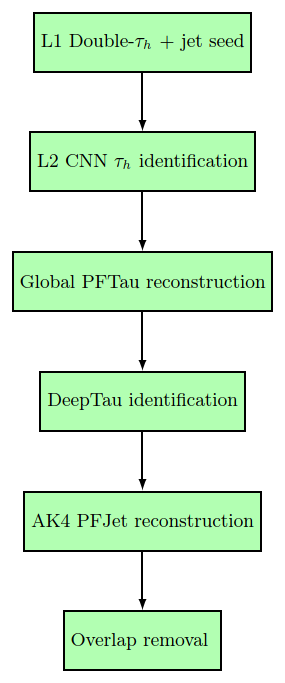
\includegraphics[width=0.4\textwidth]{Images/HLT_Path}
\end{center}
\caption{Sketch of the structure followed by the implemented HLT double-$\tau_h$ + jet path.}
\label{hh:fig:hlt_path}
\end{figure}

For an event to pass the HLT path, the first requirement is to pass the L1 seed requirements. On top of these L1 requirements, a typical HLT di-$\tau_h$ requirement is applied \cite{intro:exp:cms_trigger}: each L1 tau is used to build a Level-2 $\tau$ by associating the L1 tau all objects that fall into a $\Delta R$ cone of 0.5 with respect to it. Then, an identification algorithm based on a Convolutional Neural Network (CNN) is applied, aimed to reduce the number of background objects entering the next steps of the path (more time consuming) while reducing the least possible the number of true $\tau$ filtered. This machine learning approach is one of the new additions to Run 3 $\tau$ paths, resulting in an increase of efficiency and a decrease of rate with respect to the approaches used in the previous data-taking periods. 

After building the L2 $\tau$, global PF $\tau$ are reconstructed, similarly as how it was shown in Section~\ref{intro:subsec:taus}. Another improvement with respect to Run 3 is the use of the same \deeptau{} algorithm as in offline reconstruction level but at HLT level, resulting in better signal purity and rate reduction.

At each step, at least a pair of $\tau$ leptons needs to survive the selection. Also, the final selected $\tau$ need to match the L1 $\tau$ used for triggering at L1 within a $\Delta R$ of 0.5, and their $p_t$ must be higher than 30~GeV.

After selecting the $\tau$, the PF algorithm is used again to reconstruct the PF jets in the event. These PF jets will be selected if they satisfy an overlap removal criteria similar to the one used at L1: no matching (within a $\Delta R$ of 0.5) between the jet and a pair of PF $\tau$ that passed the whole HLT selection. On top of this criteria, the jet must match a L1 jet used for triggering and have a $p_t$ higher than a given threshold. For the main HLT path (triggered with the L1 seed with the 55~GeV $p_T$ threshold), this threshold is set to 60 GeV, while for the backup path, it is set to 75 GeV.

\section{Performance of the double-$\tau_h$ + jet HLT path}

\subsubsection{Expected rate using 2018 data}

To compute the rate expected from the addition of the new path, a similar approach than the one used in Section~\ref{hh:sec:l1seeds} is considered: the rate is estimated from a zero bias data sample taken during several 2018 runs but with Run-3 conditions applied (PU linearly scaled to 53 and 2748 colliding bunches). The rate obtained for this path is around $15.7\pm3.8$~Hz. Note that, as the expected rate by an HLT path is very small (around two to three orders of magnitude smaller than the correspondent L1 seed), a lot of zero bias events are needed to obtain a reasonably accurate result. In fact, even with all the 2018 runs that were used to obtain this value, only 15 events were able to pass the trigger, so the statistical uncertainty drives the result obtained.

For the sake of validating the result, the rate was obtained in the same sample also for the main L1 seed (\texttt{L1\_DoubleIsoTau26er2p1\_Jet55\_RmOvlp\_dR0p5}) described in Section~\ref{hh:sec:l1seeds}, resulting in a rate of 8.94~kHz, in agreement with the value obtained in that Section. 

\subsubsection{Rate using 2022 data}

In parallel to the inclusion of the new L1 double-\tauh{}+jet seed (and its backup seed) in the L1 menu, their corresponding HLT paths were also included. Fig.~\ref{hh:fig:hlt_rate_run3} shows the rate distribution for the HLT double-\tauh{}+jet path obtained from the same collision data sample used for the L1 seed rate estimation. In this case, the rate scaling with respect to PU is not as linear as for the L1 seed. However, for PU 53 we obtain a rate of around 15~kHz, in agreement with our expectation using 2018 data.

\begin{figure}[h!]
\begin{center}
\includegraphics[width=0.6\textwidth]{Images/HLT_rate}
\end{center}
\caption{HLT double-\tauh{}+jet path rate as a function of the PU for a Run 3 collision data sample collected during 2022.}
\label{hh:fig:hlt_rate_run3}
\end{figure}

\subsubsection{L1$\times$HLT efficiency}

In order for a trigger path to be used in the different analyses, the L1$\times$HLT efficiency has to be computed for both data and simulated events, so the latter can be reweighed by applying adequate scale factors. The procedure to obtain this efficiency is similar to the one shown for the L1 seeds: assuming the $\tau_h$ and jet objects are uncorrelated, the total efficiency can be computed as the product of the efficiency of selecting the leading $\tau$, the subleading $\tau$ and the jet.

The $\tau_h$ trigger efficiency can be measured through a tag-and-probe technique, as was done to compute the L1 efficiency, by selecting events that were triggered by a single-muon HLT path. Out of these events, the efficiency will be measured from the ones that also passed a HLT cross-trigger that requires a muon (used as tag) and a $\tau_h$ (used as probe). This path was implemented so that the selections applied on the muon are the same as in the single-muon path and the ones applied on the $\tau_h$ are the same requirements than in the double-$\tau_h$+jet path. The efficiency on each $\tau$ is considered as independent from the other. Fig.~\ref{hh:fig:hlt_eff_tau} shows the efficiency as a function of the $\tau_h$ $p_T$ and $\eta$ for real data collected during Run 3 and simulated events from the previous Z~+~2 jets sample. The agreement between data and simulated events is very satisfactory, and will be improved after the inclusion of an scale factor for the simulated events.

\begin{figure}[h!]
\begin{center}
\subfloat{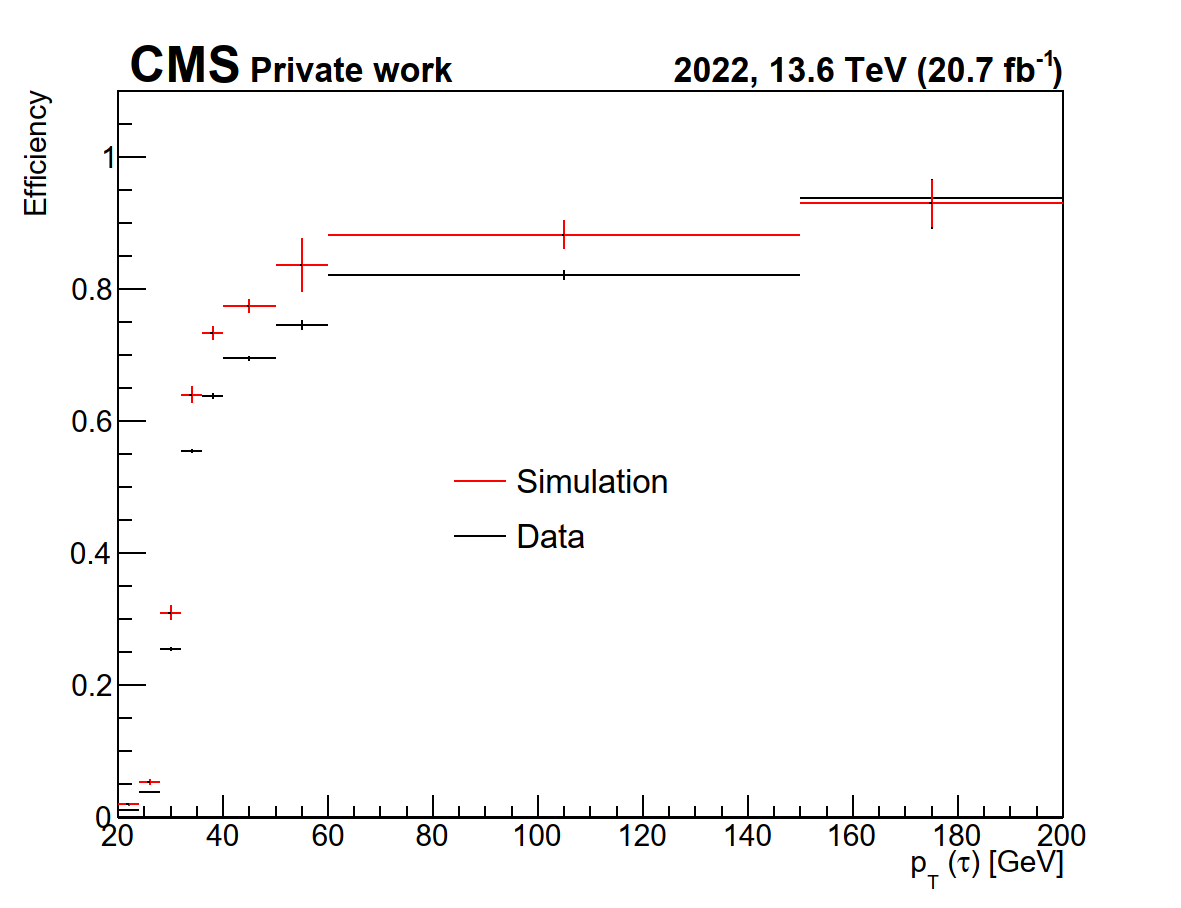
\includegraphics[width=0.49\textwidth]{Images/ditaujet_tauleg_pt}}
\subfloat{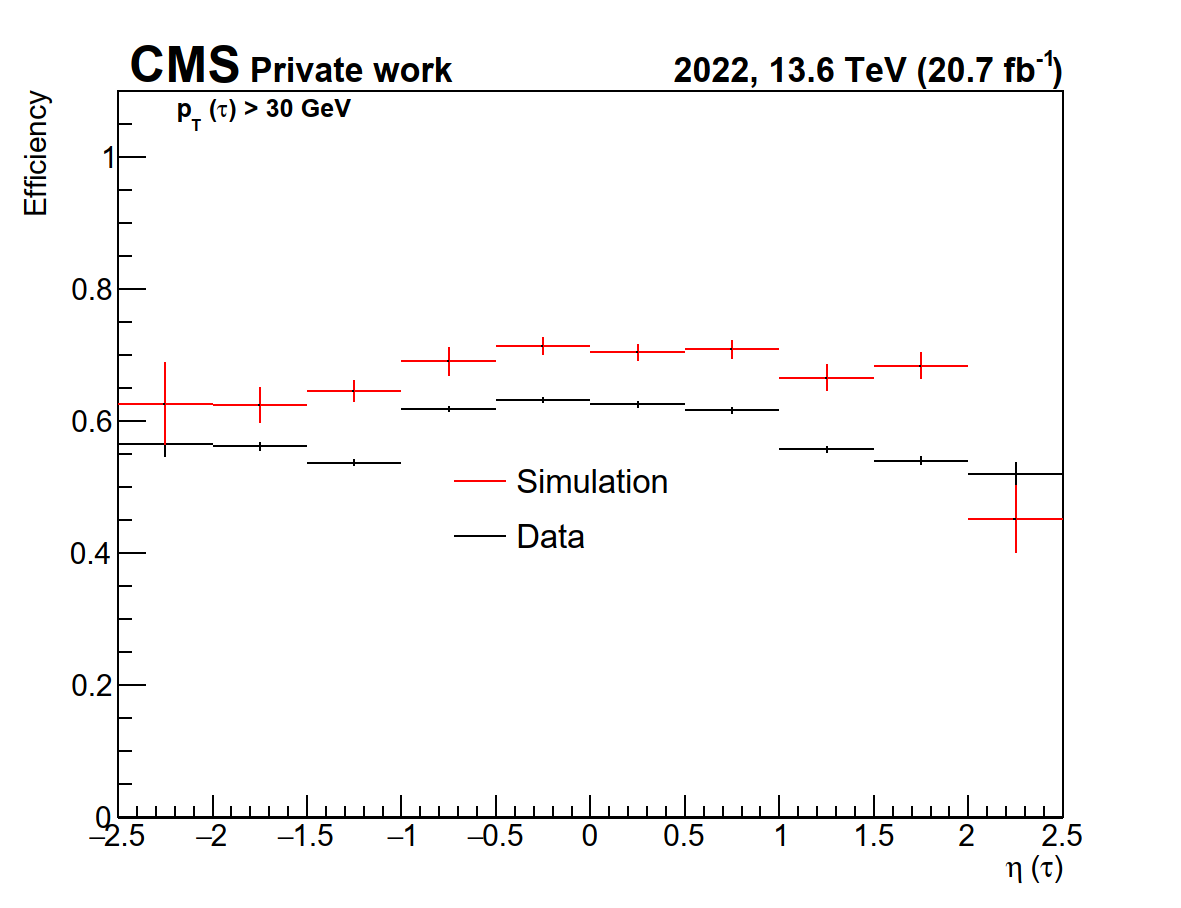
\includegraphics[width=0.49\textwidth]{Images/ditaujet_tauleg_eta}}
\end{center}
\caption{\textcolor{red}{DUMMY PLOTS} $\tau_h$ HLT trigger efficiency with respect to the offline $\tau_h$ $p_T$ (left) and $\eta$ (right) for data events collected during Run 3 (black) and simulated events from a Z~+~2 jets sample (red). Simulated events are reweighed so their PU distribution matches the one from the data. Generator-level weights are applied to the simulated events.}
\label{hh:fig:hlt_eff_tau}
\end{figure}

In a similar way, the jet trigger efficiency is measured by selecting events with one muon, at least one $\tau_h$ and at least one jet that were triggered by the muon-$\tau_h$ cross-trigger. Out of these events, the efficiency will be computed from the ones that were triggered by an HLT muon-$\tau_h$-jet cross trigger, where the requirements on the trigger muon and $\tau_h$ are the same as in the muon-$\tau_h$ cross trigger and the requirements on the jet are the same as in the double-$\tau_h$+jet trigger. Fig.~\ref{hh:fig:hlt_eff_jet} shows the efficiency as a function of the jet $p_T$ and $\eta$ for real data collected during Run 3 and simulated events from the previous Z~+~2 jets sample. The agreement between data and simulated events is even better than for the $\tau_h$.

\begin{figure}[h!]
\begin{center}
\subfloat{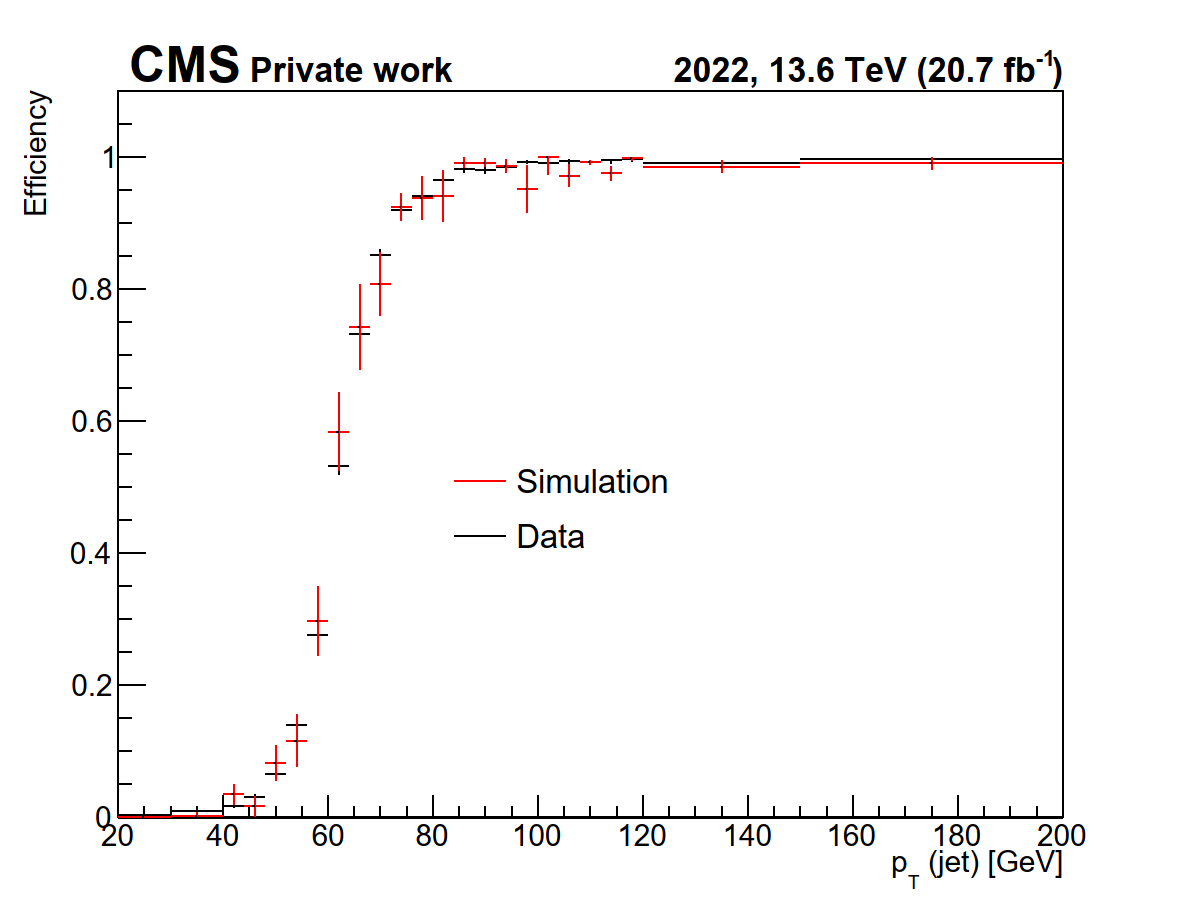
\includegraphics[width=0.49\textwidth]{Images/ditaujet_jetleg_pt}}
\subfloat{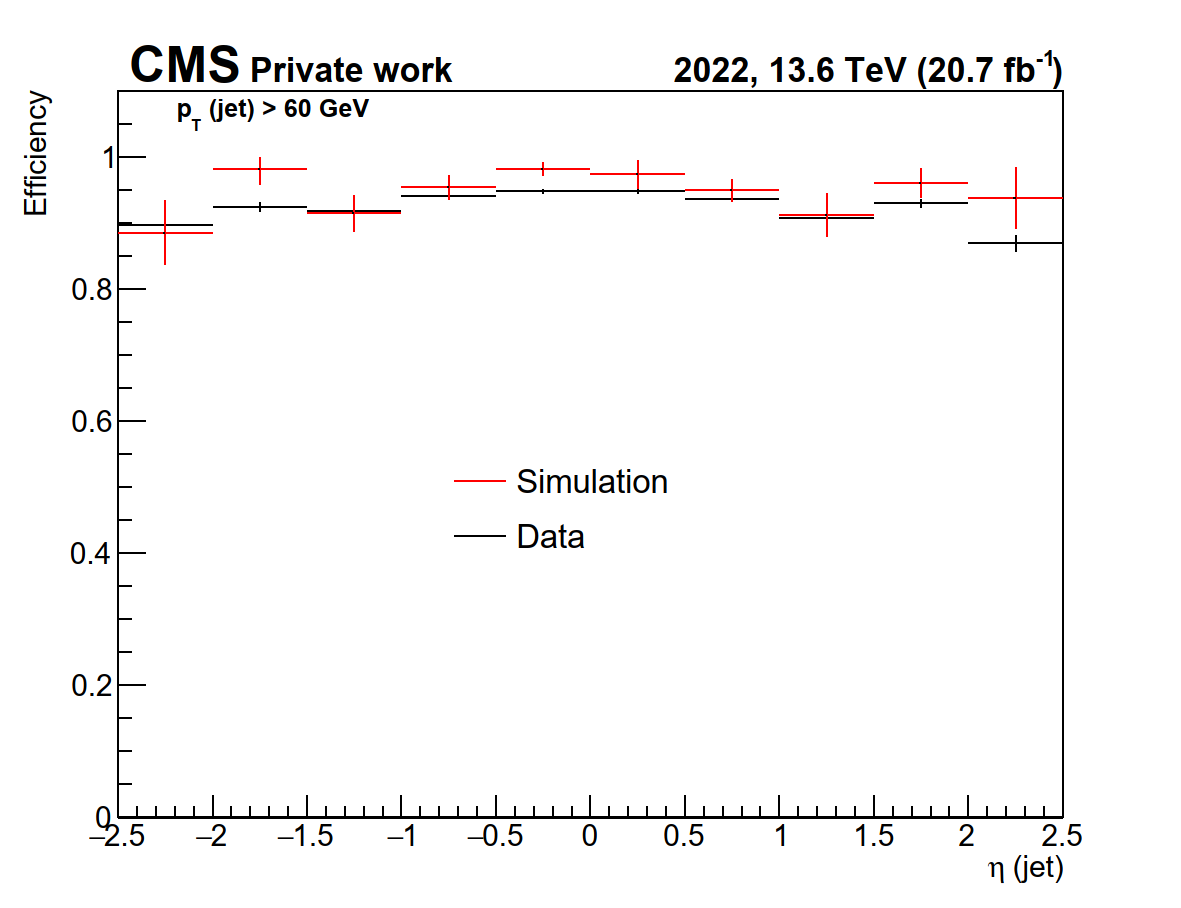
\includegraphics[width=0.49\textwidth]{Images/ditaujet_jetleg_eta}}
\end{center}
\caption{\textcolor{red}{DUMMY PLOTS} Jet HLT trigger efficiency with respect to the offline jet $p_T$ (left) and $\eta$ (right) for data events collected during Run 3 (black) and simulated events from a Z~+~2 jets sample (red). Simulated events are reweighed so their PU distribution matches the one from the data. Generator-level weights are applied to the simulated events.}
\label{hh:fig:hlt_eff_tau}
\end{figure}


%\bibliographystyle{plain}
%\bibliography{../biblio.bib}





\end{document}

